\subsection{Interrupts from the JTAG* UART}

Figure \ref{fig:jtag_port}, reproduced as Figure \ref{fig:jtag_port_int}, shows the {\it Data} 
and {\it Control} registers of the JTAG UART. As we said in Section~\ref{sec:jtag_port}, 
{\it RAVAIL} in the {\it Data} register gives the number of characters that 
are stored in the receive 
FIFO, and {\it WSPACE} gives the amount of unused space that is available in the transmit FIFO. 
The {\it RE} and {\it WE} bits in Figure \ref{fig:jtag_port_int}
are used to enable processor interrupts associated with the receive and transmit FIFOs. 
When enabled, interrupts are generated when {\it RAVAIL} for the receive FIFO, 
or {\it WSPACE} for the transmit FIFO, exceeds 7. Pending interrupts are indicated in the 
Control register's {\it RI} and {\it WI} bits, and can be cleared by writing or reading data
to/from the JTAG UART.

\begin{figure}[h!]
   \begin{center}
       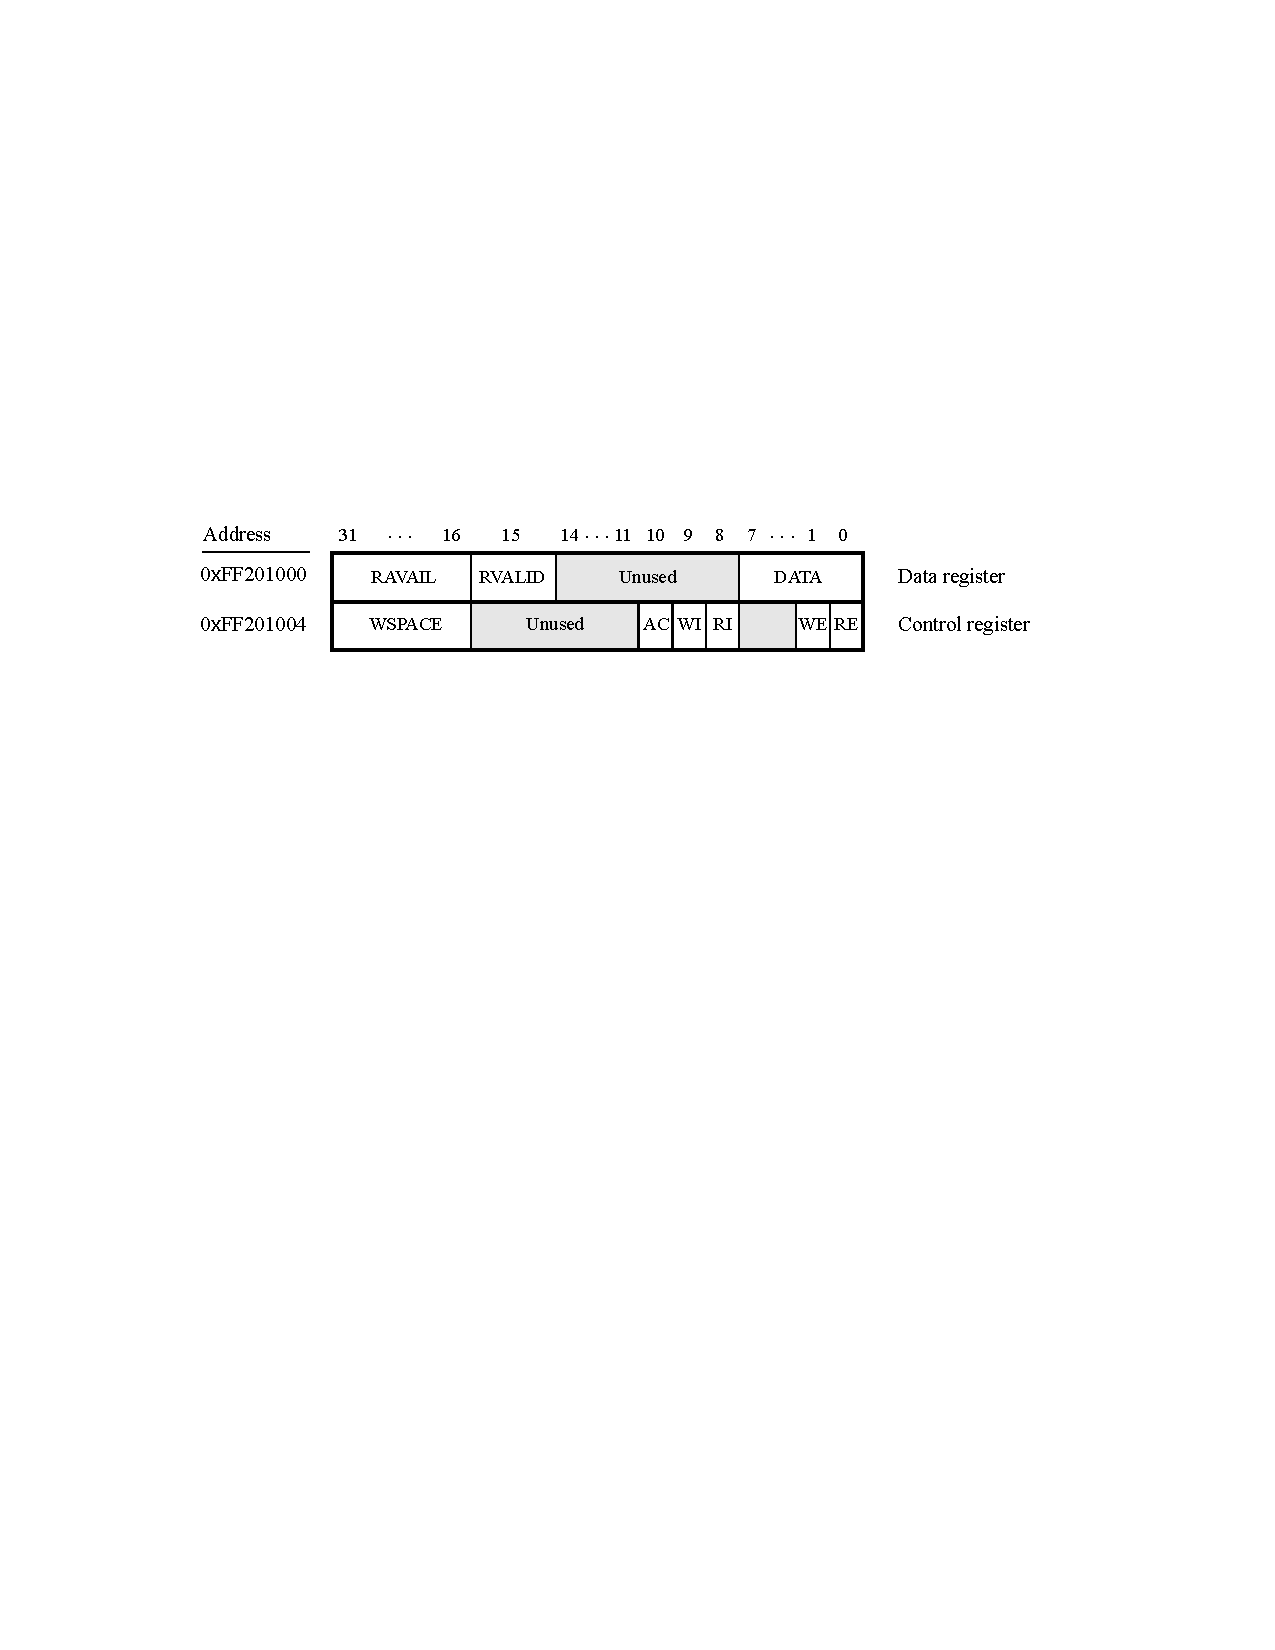
\includegraphics{../../../common/figs/FPGA_JTAG_UART.pdf}
   \end{center}
   \caption{Interrupt bits in the JTAG UART registers.}
	\label{fig:jtag_port_int}
\end{figure}


